\documentclass{llncs}

\usepackage{forest}
\usepackage[utf8]{inputenc}
\usepackage{listings}
\usepackage{hyperref}
\usepackage{algpseudocode}
\usepackage{minibox}

\graphicspath{{./img_t2/}}


\definecolor{folderbg}{RGB}{124,166,198}
\definecolor{folderborder}{RGB}{110,144,169}
\def\Size{4pt}
\tikzset{
      folder/.pic={
        \filldraw[draw=folderborder,top color=folderbg!50,bottom color=folderbg]
          (-1.05*\Size,0.2\Size+5pt) rectangle ++(.75*\Size,-0.2\Size-5pt);  
        \filldraw[draw=folderborder,top color=folderbg!50,bottom color=folderbg]
          (-1.15*\Size,-\Size) rectangle (1.15*\Size,\Size);
      }
    }





\begin{document}

\title{Relatório do Trabalho 3}
\author{Gustavo Henrique Fernandes Carvalho - 14/0021671}
\institute{Fundamentos Computacionais de Robótica - 2017/2 - Universidade de Brasília}
\maketitle


O video da simulação está em \url{https://youtu.be/S3OfUqVDY18}


\section{Informações do pacote}
\subsection{Dependências}
As dependências do nó principal do trabalho 3 estão definidas no arquivo \textit{package.xml} do pacote \textit{fcr2017}.

Para visualizar o gráfico de probabilidades em tempo real é necessário ter instalado a biblioteca Matplotlib do Python, ela já vem instalada na maioria das distribuições do Python.


\subsection{Rodando a simulação} \label{sec:run}
Para rodar a simulação é necessário apenas executar o seguinte comando no terminal:
\begin{lstlisting}[language=bash]
	$ roslaunch fcr2017 trabalho3.launch
\end{lstlisting}
O arquivo \textit{trabalho3.launch} já inicia todos os nós e scripts necessários para a simulação. Mais detalhes de como interagir com a simulação são discutidos na seção \ref{sec:io}.



\subsection{Arquivos}
A Figura \ref{file_tree} mostra os novos arquivos do pacote fcr2017 utilizados para a realização do trabalho 3, os arquivos não utilizados na simulação desse trabalho e os originais do pacote não são mostrados.


\begin{figure}[h!]
\begin{forest}
      for tree={
        font=\ttfamily,
        grow'=0,
        child anchor=west,
        parent anchor=south,
        anchor=west,
        calign=first,
        inner xsep=7pt,
        edge path={
          \noexpand\path [draw, \forestoption{edge}]
          (!u.south west) +(7.5pt,0) |- (.child anchor) pic {folder} \forestoption{edge label};
        },
        % style for your file node 
        file/.style={edge path={\noexpand\path [draw, \forestoption{edge}]
          (!u.south west) +(7.5pt,0) |- (.child anchor) \forestoption{edge label};},
          inner xsep=2pt,font=\scriptsize\ttfamily
                     },
        before typesetting nodes={
          if n=1
            {insert before={[,phantom]}}
            {}
        },
        fit=band,
        before computing xy={l=15pt},
      }  
	[fcr2017
		[include - Definição de funções e estruturas em C++
			[..., file]
		]
		[launch
			[trabalho3.launch - Utilizado para iniciar a simulação, file]
			[..., file]
		]
		[src
			[140021671\_Trabalho3.cpp - Código fonte principal do trabalho 3, file]
			[common\_lib - Biblioteca implementada para facilitar o reuso e modificação do código
				[common.cpp - Funções gerais, file]
				[feature.cpp - Funções de extração de características, file]
				[laser\_sensor.cpp - Funções que manipulam os dados do sensor laser, file]
				[localization.cpp - Funções que calculam a probabilidade do Pionner está em um nó específico, file]
				[user\_motion\_controller.cpp - Controla o movimento do Pionner de acordo com os comando do usuário, file]
			]
		]
		[scripts - Nós auxiliares feitos em Python
			[140021671\_Trabalho3.cpp - Código fonte principal do trabalho 3, file]
		]
		[README.md - Mais informações sobre o pacote, file]
		[Probability.txt - Resultado do caculo da probabilidade de cada nó a cada instante de tempo, file]
		[..., file]
	]
\end{forest}
\caption{Estrutura dos arquivos.}
\label{file_tree}
\end{figure}


\section{Entrada e saída} \label{sec:io}
Ao iniciar a simulação são abertas várias novas janelas, o comportamento de cada uma delas é discutido a seguir.

\subsection{Controle de movimento} \label{sec:controller}
O controle de movimento é realizado pelo script controller.py, esse nó é iniciado em um novo terminal como na figura \ref{fig:controller}. Com ele selecionado o usuário pode utilizar as teclas 'a', 'q', 'w', 'e' e 'd' para controlar o movimento do Pionner, a tecla 's' para parar o Pionner e a tecla 'r' para reiniciar as probabilidades de cada nó.

\begin{figure}
	\centerline{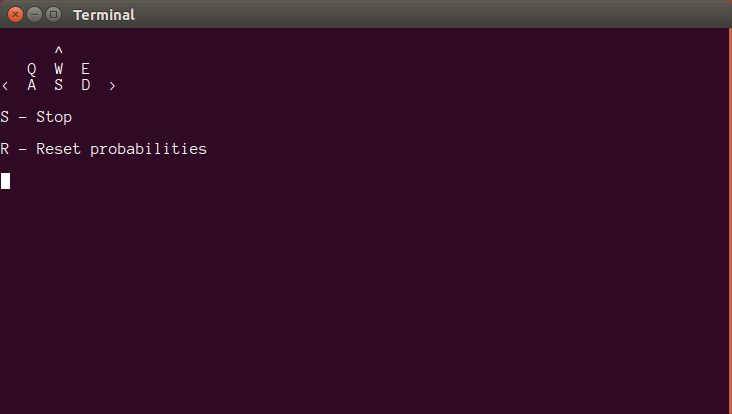
\includegraphics[scale=0.4]{controller}}
	\caption{Controle de movimento do Pionner}
	\label{fig:controller}
\end{figure}


\subsection{Gráfico de probabilidades}
O script live\_plot.py é um nó que abre uma janela com um gráfico que é atualizado em tempo real sempre que o vetor de probabilidades é recalculado, um exemplo de gráfico é mostrado na figura \ref{fig:graph}.

\begin{figure}
	\centerline{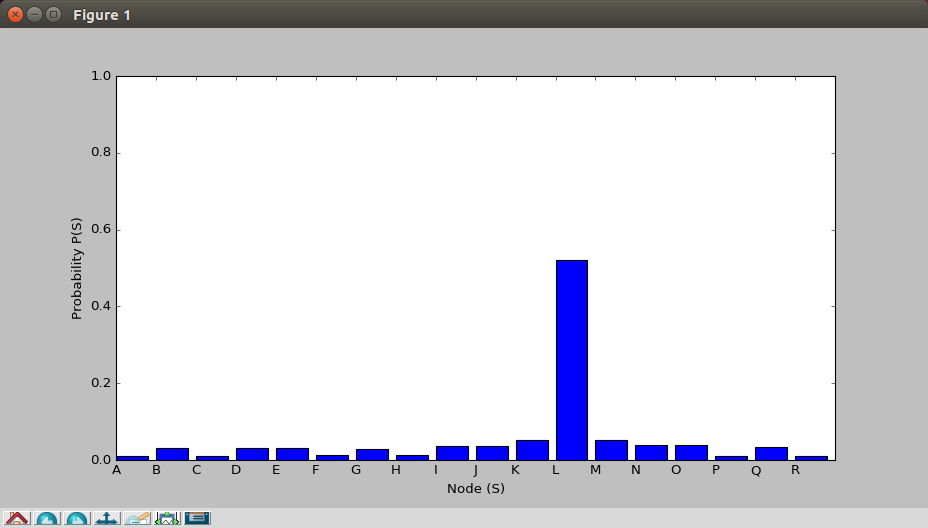
\includegraphics[scale=0.4]{graph}}
	\caption{Representação gráfica do vetor de probabilidades}
	\label{fig:graph}
\end{figure}


\subsection{Arquivo de saída}
É gerado um arquivo texto (\textit{Probability.txt}) com a evolução do vetor de probabilidades ao longo da simulação, para cada conjunto de dados do vetor também é armazenado a 'hora' da simulação em que ocorreu o cálculo, essa informação é obtida pelo comando \textit{rospy.get\_time()} e é utilizada para plotar o gráfico.

A figura \ref{fig:prob} mostra um exemplo de registro feito no arquivo, onde o primeiro número é a hora na simulação.

\begin{figure}
\label{fig:prob}
\caption{Registro de probabilidades feitas na hora 422.0 da simulação.}
\centerline{\minibox[frame]{
422.0\\
P(S = A): 0.00932169379275\\
P(S = B): 0.0320624351116\\
P(S = C): 0.00932169379275\\
P(S = D): 0.0304589829606\\
P(S = E): 0.0304589829606\\
P(S = F): 0.0121541121012\\
P(S = G): 0.0288555308096\\
P(S = H): 0.0121541121012\\
P(S = I): 0.0375567197768\\
P(S = J): 0.0375567197768\\
P(S = K): 0.0529888911995\\
P(S = L): 0.52209071541\\
P(S = M): 0.0529888911995\\
P(S = N): 0.0395158845266\\
P(S = O): 0.0395158845266\\
P(S = P): 0.0101124448224\\
P(S = Q): 0.0327738603093\\
P(S = R): 0.0101124448224
}}
\end{figure}


\section{Algoritmos}

\subsection{Desvio de obstáculo}
Como é o usuário que controla totalmente o movimento do Pionner não foi implementado nenhum algoritmo para contornar obstáculos, porém o controle de movimento ainda impede que o Pioneer colida com qualquer objeto impedindo o movimento quando ele chega muito perto de um objeto e então a única ação que o usuário pode executar é girar o Pionner até que a frente esteja livre.

\subsection{Extração de características}
A extração de características utiliza as leituras do pacote \textit{laser line extraction} identificando retas com pontos ou inclinações em comum e determinando se elas formam um corredor, canto interno, canto externo ou interseção.

Quando um corredor é identificado o algoritmo verifica se o Pionner está dentro do corredor é calcula a largura do corredor.

Ao identificar um canto, isto é, duas retas com um ponto em comum e um ângulo de aproximadamente 90 graus, o canto é classificado como interno caso o ponto não comum entre as retas está mais próximo do Pionner que o ponto em comum, caso contrario o canto é considerado externo. Se dois cantos são identificados e uma reta de um canto está alinhada com a reta do outro canto então uma interseção é identificada.

\subsection{Cálculo da probabilidade}
O cálculo da probabilidade do Pionner estar em um nó especifico é dividido em duas etapas, a primeira é a fase de predição do filtro, pela equação \ref{fig:eq1}.

\begin{figure}
	\centerline{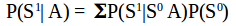
\includegraphics[scale=0.7]{eq1}}
	\caption{Fase de predição do filtro}
	\label{fig:eq1}
\end{figure}

Nessa fase é utilizado uma matriz de probabilidade de dado um nó S0 qual é a probabilidade do Pionner se mover do S0 para um nó S1 qualquer.

A segunda fase do calculo da probabilidade leva em consideração o processamento das características identificadas com o modelo de percepção dado pela equação \ref{fig:eq2}.

\begin{figure}
	\centerline{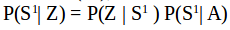
\includegraphics[scale=0.7]{eq2}}
	\caption{Modelo de percepção}
	\label{fig:eq2}
\end{figure}

Nesse modelo é levado em consideração a probabilidade do Pionner ver cada uma das características em um nó específico e também o vetor de probabilidade calculado na fase anterior.


\section{Conclusão}
O trabalho apresentou grandes desafios na implementação do cálculo de probabilidades e extração de características. Os algorítimos implementados em geral funcionaram conforme o esperado, porém em alguns casos específicos foi identificado alguns erros na determinação se o canto é interno ou externo e no reconhecimento de interseções.



\begin{thebibliography}{9}

\bibitem{AI}
	Robin R. Murphy. 2000,
	Introduction to AI Robotics (1st ed.),
	MIT Press, Cambridge, MA, USA. 
	
\bibitem{slides}
	Carla Koike,
	Slides da disciplina Fundamentos Computacionais de Robótica,
	Departamento de Ciência da Computação, UnB.
	
\bibitem{primer}
	Maja J. Matarić,
	The Robotics Primer,
	MIT Press.
	
\bibitem{git}
	https://github.com/kam3k/laser\_line\_extraction

\end{thebibliography}

\end{document}
